\begin{savequote}[8cm]
Simplicity is prerequisite for reliability.
  \qauthor{--- Edsger W. Dijkstra}
\end{savequote}

\chapter{High-level modular assembly}

Already from the start, the field of structural DNA nanotechnology has been interested in modular assemblies, although mostly in the form of infinite chrystal structures. Allegedly, Ned Seeman was inspired to pioneer the field after seeing the artwork Depth my M.C. Escher.

This chapter will provide an overview on the background of multi-component assemblies, starting with experimental results of ever-increasing size and followed by a selection of theoretical models.

\section{Experimental applications} \label{sec:experimental_appl}
There is an increasing interest within the field of DNA nanotechnology to create finite-sized multi-component objects.
\subsection{DNA tiles and bricks}

\subsection{RNA tiles}
In 2014, Cody Geary published a method of folding RNA tiles co-transcriptionally \cite{geary2014single}. The design used a set of tertiary RNA motifs, such as kissing hairpins and double crossovers, to fold the DNA helices into the desired tile structure. The tiles then assembled connected by complementary 120-degree kissing loop interactions. The design method was later described in depth in the \emph{Methods in Molecular Biology} book series \cite{sparvath2017computer}.

\subsection{DNA origami arrays}
% https://www.nature.com/articles/nature24655

In 2007, Tikhomirov, et al.\cite{tikhomirov2017fractal} demonstrated two-dimensional patterns assembled on the micrometre-scale using square origami tiles connecting through their complementary edges. 

\subsection{Shape-complementary origami}
% 2D https://www.nature.com/articles/nchem.1070
% 3D https://science.sciencemag.org/content/347/6229/1446.abstract

Also in 2007, Wagenbauer, et al. \cite{wagenbauer2017gigadalton} used shape-complementarity to assemble origami tiles into three-dimensional polyhedral shapes up to 450 nanometers in diameter.

\subsection{Octahedral DNA origami frames}
% https://onlinelibrary.wiley.com/doi/abs/10.1002/anie.201913958

\subsection{DNA origami nanochambers}
% https://pubs.acs.org/doi/full/10.1021/jacs.0c07263

\section{Tile assembly models}
It would be computationally unreasonable to simulate module assembly at the level of individual nucleotides. A better approach is instead to use an abstract model to predict the assembly process with the modules treated as rigid bodies. This section will present two such models as a background to my own model described in Chapter \ref{ch:3-polycubes}.

%\subsection{Wang tiles}

\subsection{The algorithmic tile assembly model}

% David Doty overview: https://cacm.acm.org/magazines/2012/12/157881-theory-of-algorithmic-self-assembly/fulltext

In his 1998 thesis Erik Winfree showed the usage of the double-crossover (DX) motif to create regular arrays \cite{winfree1998design}. These tiles behave like Wang tiles\cite{wang1961proving} and do not allow rotations or reflections. Winfree also investigated the possibility of using such tiles for computation \cite{winfree1998algorithmic}.
% DX array https://www.nature.com/articles/28998

Co-operative binding

\subsection{The polyomino model}

The main difference to aTAM is that polyomino tiles are allowed to rotate. They also have a constant binding strength (in other words, it is a temperature-1 model).

A past venture in this direction is Iain Johnston's research on two-dimensional assembly\cite{ahnert2010self}\cite{johnston2011evolutionary}, studying the self-assembly, modularity and evolutionary dynamics of \emph{polyominoes}.

Polyominoes are abstract structures composed of one or more squares, connected by their edges. The polyomino assembly model developed by Johnston is similar in assembly to the later micro-meter scale tile designs by Tikhomirov \cite{tikhomirov2017fractal} described earlier. These polyomino tiles differ from Wang tiles\cite{wang1961proving} in that edge binding does not need to be between edges of the same colour, but can be specified by a more complex interaction matrix. Furthermore, the tiles can be rotated to bind, creating further possibilities for symmetries.

\begin{figure}[h]
    \centering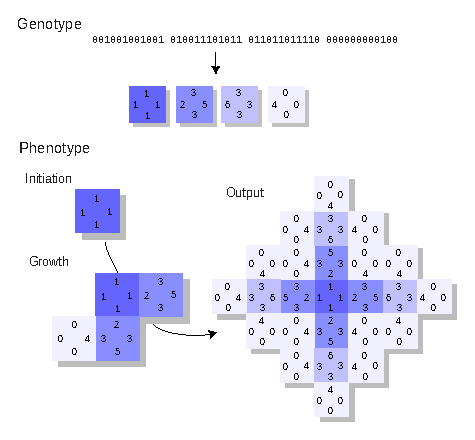
\includegraphics[width=0.6\textwidth]{figures/polyominoes.eps}
    \caption{Illustration of the polyomino assembly model used by Johnston. A \emph{genotype}, in the form of a ruleset of possible tiles, encodes for a polyomino \emph{phenotype}, grown stochastically from an initial seed tile. Image adapted from \cite{johnston2011evolutionary}.}
    \label{fig:polyominoes}
\end{figure}

I aim to build on Johnston's work on polyominoes to explore the properties of such self-assembling systems in three dimensions; the self-assembly of \emph{polycubes}. With such a model in place, it should be possible to design, through shape complementary in DNA origami \cite{wagenbauer2017gigadalton}, kissing interactions in RNA origami \cite{geary2014single}, or other methods, robotic modules with the interfaces necessary to assemble into the desired polycube shape. My current progress within this project is covered in Chapter \ref{ch:3-polycubes}.

\section{Algorithmic Information Theory and input-output maps}

\section{Patchy particle simulation}
